\section*{Methodology}
\addcontentsline{toc}{section}{Methodology}

\subsection*{Research Design}
This thesis applies a qualitative, theory-building comparative case study 
design (\cite{George2005}). Germany and Chile are selected as ``most different systems'' 
facing similar biophysical pressures but embedded in contrasting political–institutional 
contexts. This design maximizes analytical leverage by exploring how structural 
differences condition actor strategies. 

\textbf{Germany} represents a corporatist welfare state with high institutional density 
and a tradition of consensus-oriented forestry. \textbf{Chile}, in contrast, embodies a 
neoliberal state with fragmented authority, powerful private-sector actors, and persistent 
socio-environmental conflicts. Comparing these two cases enables identification of how 
divergent legacies shape the room for maneuver of ideational actors.

\subsection*{Operationalization of the ``Ideational Bricoleur''}
A core innovation of this study is the operational definition of the 
\textbf{ideational bricoleur}. An actor (organization, coalition, or individual) 
is coded as a bricoleur when all three conditions are observed in the corpus:

\begin{enumerate}
    \item \textbf{Discursive recombination:} The actor explicitly combines elements from 
    at least two distinct or competing discourses (e.g., climate-smart forestry + 
    indigenous territorial rights).
    \item \textbf{Institutional patching:} The actor proposes connecting or adapting 
    institutional tools from different domains (e.g., linking market certification 
    with community-based forest management).
    \item \textbf{Strategic intent:} The actor frames this recombination as a solution 
    to adaptation, signaling intent to influence policy trajectories rather than merely 
    describe problems.
\end{enumerate}

If all three criteria are met in at least two independent documents, the actor will 
be categorized as an \textit{ideational bricoleur}. This threshold follows a reliability 
logic: multiple independent appearances reduce the likelihood of spurious classification. 
Future research could strengthen this with triangulation (e.g., interviews, meeting minutes, media coverage).

\smallskip
This operationalization represents a methodological innovation: it provides a 
replicable coding protocol for comparative North–South adaptation studies, 
allowing future research to systematically test, extend, or challenge the 
bricoleur concept in other governance domains.


\subsection*{Operationalizing Observable Uptake}

Effectiveness of bricolage is defined not by intent alone but by \textbf{observable uptake} 
in governance processes. To ensure analytical rigor, uptake is measured using a 
multi-dimensional index with four concrete indicators. Each indicator is coded as binary (0/1), 
with a cumulative score from 0--4. This allows both cross-actor and cross-country comparison.

\begin{enumerate}
    \item \textbf{Textual reuse in official policy drafts or laws.}  
    Evidence that specific frames or instruments promoted by an actor appear verbatim 
    or paraphrased in draft legislation, decrees, or official strategies.

    \item \textbf{Resource allocation (funding or pilot programs).}  
    Identification of cases where bricolage proposals are linked to concrete 
    funding decisions (e.g., subsidies, grants, pilot initiatives) in government or 
    international donor budgets.

    \item \textbf{Institutional incorporation.}  
    Uptake operationalized as inclusion of bricolage elements in the mandates, 
    procedures, or reporting frameworks of public agencies, advisory councils, or 
    certification bodies.

    \item \textbf{Actor representation in decision venues.}  
    Evidence that proponents of bricolage strategies gain seats, speaking roles, 
    or formal recognition in decision-making arenas (e.g., parliamentary hearings, 
    advisory committees, certification governance boards).
\end{enumerate}

\textbf{Scoring:}  
Each bricolage strategy receives one point per indicator satisfied. A score of 0 
denotes no observable uptake; a score of 4 indicates full incorporation across 
multiple dimensions. This index allows both within-case and cross-case comparison, 
making uptake claims transparent and replicable.

\textbf{Reliability:}  
Coding for uptake will follow a double-check protocol. If uptake evidence is 
ambiguous (e.g., partial text reuse), coders must document justification in 
memos and subject the case to a second review. Cohen’s $\kappa$ will be 
calculated on a 15\% subsample to ensure intercoder reliability, with a 
target threshold of $\kappa \geq 0.7$.

\subsection*{Data Collection and Sources}
The analysis will rely on a document corpus produced between 2015 and 2025, 
covering the post-Paris Agreement decade of intense adaptation policy development. 
The corpus includes:

\begin{itemize}
    \item \textbf{Core policy documents:} National adaptation strategies 
    (DE: DAS 2024; CL: ENCCRV, Plan de Adaptación Forestal) and climate legislation 
    (DE: KSG; CL: Ley Marco de Cambio Climático).
    \item \textbf{Grey literature:} Policy briefs, position papers, and manifestos 
    from NGOs, industry associations, and professional organizations.
    \item \textbf{Scientific and technical reports:} For Germany, outputs from Thünen, EFI, and 
    federal agencies. For Chile, a carefully selected subset of CONAF and MMA reports, complemented 
    by recent scientific contributions on hydrology, wildfires, and biodiversity. 
    This targeted approach ensures grounding without aiming for exhaustive coverage.
    \item \textbf{Public communication:} Media articles, press releases, and 
    parliamentary debates reflecting the communicative discourse.
\end{itemize}

\textit{Inclusion criteria:} documents published between 2015–2025, explicitly addressing 
forest adaptation or governance debates, and originating from state, NGO, industry, or academic actors.  
\textit{Exclusion criteria:} purely technical reports without governance content, duplicates, 
and journalistic sources not citing actor positions.
\smallskip
While the study relies exclusively on documents, triangulation across policy, 
grey literature, and media sources captures both elite and public discourse, 
helping mitigate the absence of interviews.

\subsection*{Corpus Construction and Feasibility}

The document corpus is deliberately scoped to ensure analytical depth within the 
accelerated timeline. Rather than aiming for exhaustive national coverage, the corpus 
is structured as a tiered and capped selection:

\begin{enumerate}
    \item \textbf{Primary corpus (30--40 documents per country).}  
    Includes high-salience laws, national strategies, and major policy briefs 
    from state agencies, NGOs, and industry associations. These represent the 
    core discursive arenas where bricolage strategies are most visible.

    \item \textbf{Secondary corpus (triangulation only).}  
    Selected grey literature and media documents are consulted for contextualization 
    but not coded systematically. Their role is to triangulate findings and enrich 
    interpretation, not to expand the coded dataset.
\end{enumerate}

This tiered strategy balances feasibility with theoretical leverage: it treats 
documents as ideal-typical evidence of discursive and institutional strategies, 
not as a census of all adaptation texts. By capping the corpus at approximately 
80 systematically coded documents, the design avoids superficial coding and 
ensures that comparative insights remain analytically robust and defensible 
within the timeframe.

\textit{Inclusion criteria:} (i) documents explicitly addressing forest adaptation 
or governance debates, (ii) produced by state, NGO, industry, or academic actors.  
\textit{Exclusion criteria:} purely technical or scientific reports without 
governance content, duplicates, and journalistic texts not attributing positions 
to identifiable actors.

%\begin{figure}[h!]
%\centering
%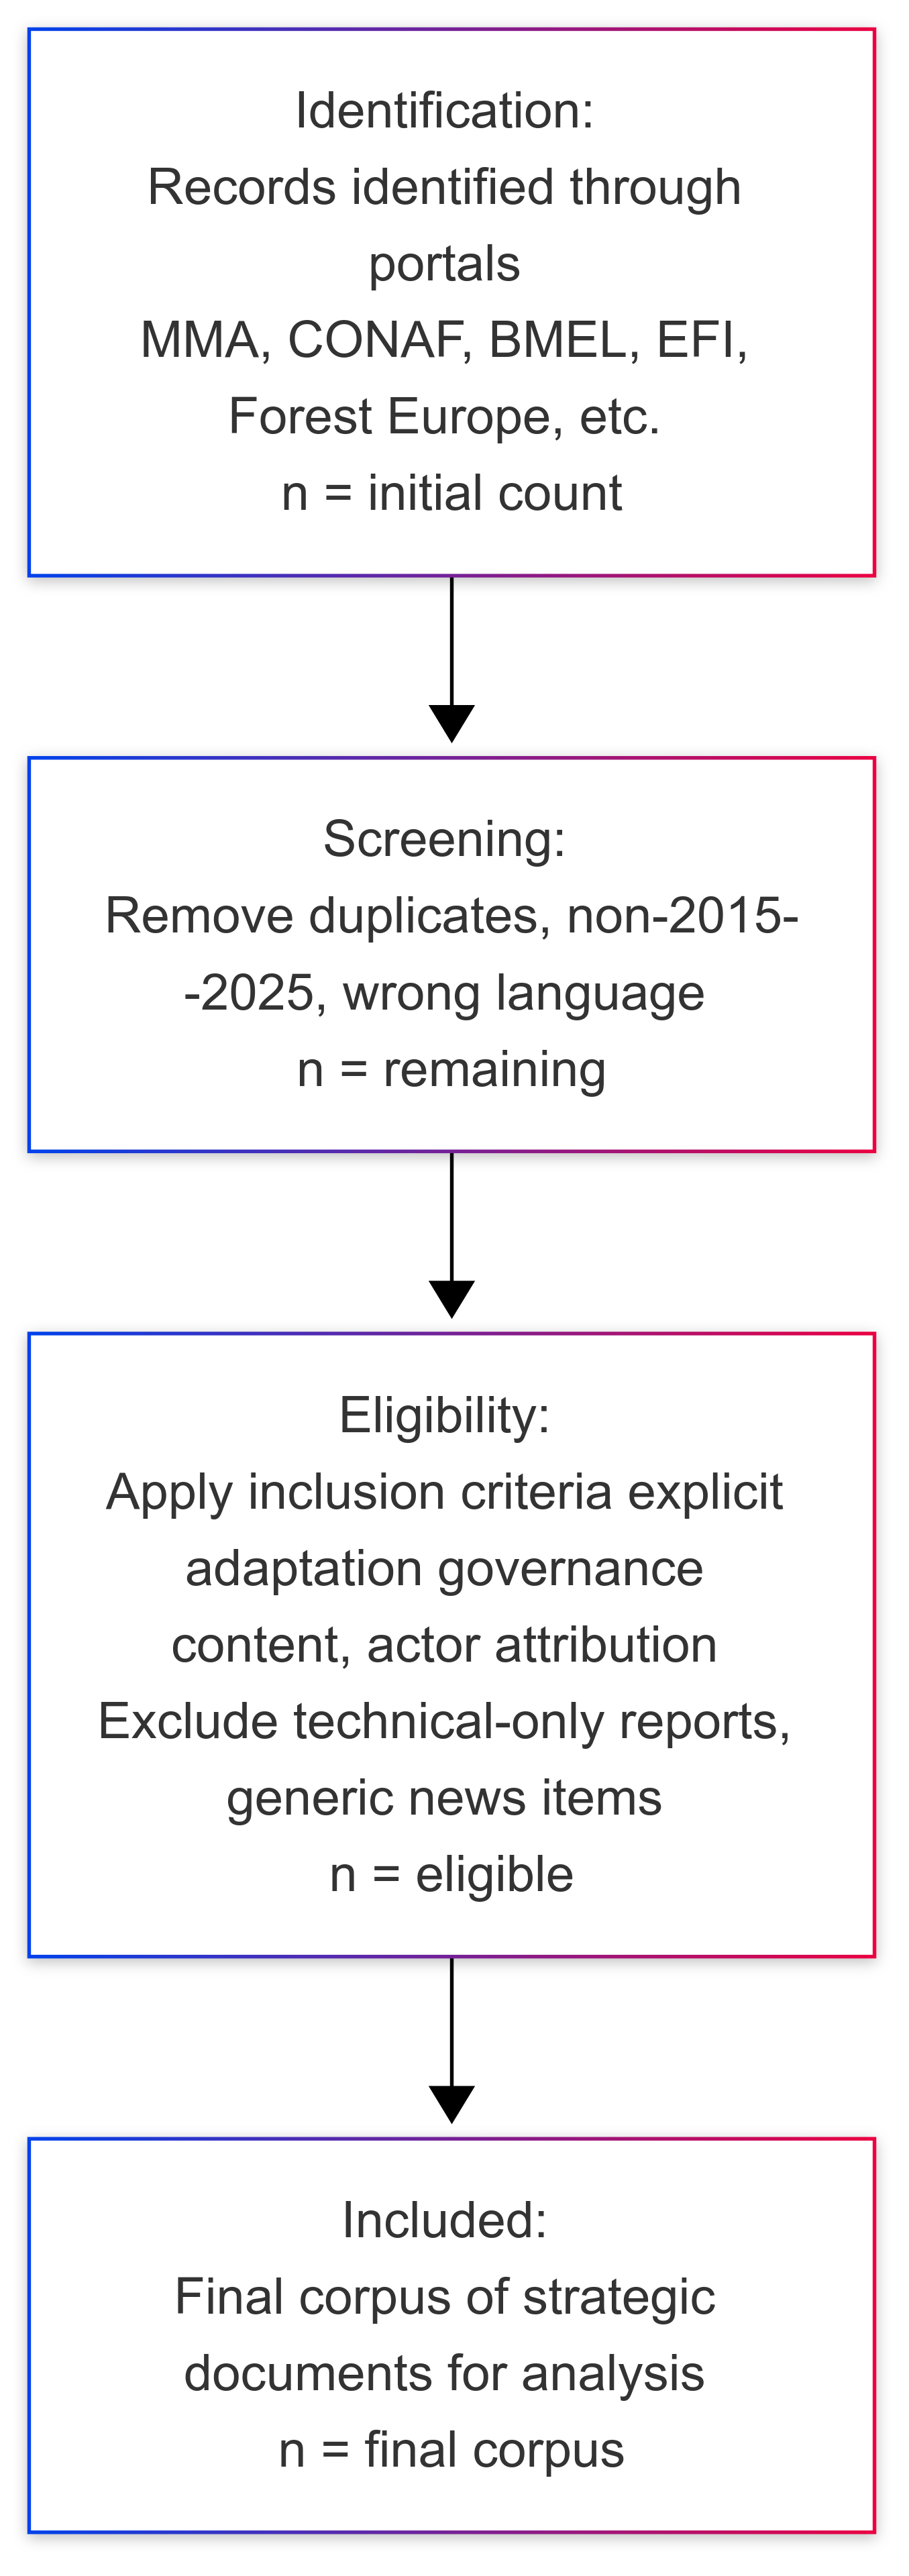
\includegraphics[width=0.4\textwidth]{src/fig/prisma.png}
%\caption{PRISMA-style flow diagram for corpus construction. 
%The figure illustrates the sequential filtering of documents from initial identification 
%through screening, eligibility assessment, and final inclusion. Numbers in brackets 
%($n = \ldots$) will be updated once the corpus is finalized.}
%\label{fig:prisma-flow}
%\end{figure}

\subsection*{Unit of Analysis and Actor Universe}

The unit of analysis is the \textbf{strategic document} (laws, strategies, policy 
briefs, manifestos, reports).  
Actors are coded according to organizational type: NGOs, community organizations, 
industry associations, professional forestry bodies, and state agencies. This 
prevents sampling on the dependent variable and provides a replicable frame 
for actor selection.



\subsection*{Coding Protocol (Codebook)}

Each document is coded according to a one-page codebook with three binary indicators:

\begin{enumerate}
    \item \textbf{Discursive recombination:} presence of explicit co-reference 
    to at least two distinct discourse families (e.g., climate-smart forestry 
    + territorial rights).
    \item \textbf{Institutional patching:} reference to the combined or adapted 
    use of distinct institutional instruments (e.g., subsidy scheme + certification standard).
    \item \textbf{Strategic intent:} proposal linked to a concrete governance 
    decision, venue, or policy trajectory.
\end{enumerate}

An actor is classified as an \textit{ideational bricoleur} if all three 
conditions are met across at least two independent documents. This threshold 
follows a reliability logic: multiple independent appearances reduce spurious 
identification.



\subsection*{Reliability Procedures}

To address coder bias, the following measures are implemented:

\begin{itemize}
    \item Code--recode reliability: a 15\% subsample of documents will be re-coded after a two-week interval.
    \item Cohen’s $\kappa$ will be calculated on this subsample to quantify reliability. 
    \item All coding will be documented through memos and an audit trail stored in the project’s repository.
\end{itemize}



\subsection*{Recognized Limitation}

The analysis captures \textbf{documented strategies}, not actor intentions. Strategic 
intent is inferred from textual claims targeting governance decisions, not from 
cognitive or motivational states. This scoping choice ensures feasibility and 
methodological defensibility while leaving open future triangulation with interviews.

\textit{Limitation:} No interviews are included due to time constraints. However, 
triangulation across policy, grey, and media sources captures both elite 
(coordinative) and public (communicative) discourse, providing a robust basis for 
analysis.   


\subsection*{Analytical Framework}
The analysis proceeds in three stages, each with clear coding procedures.

\begin{enumerate}
    \item \textbf{Stage 1: Actor and Frame Identification.}  
    Using frame analysis, all documents will be coded for:
    \begin{itemize}
        \item \textit{Diagnostic frame:} Problem definition (e.g., ``forest death'', 
        ``violation of rights'').
        \item \textit{Prognostic frame:} Proposed solutions (e.g., 
        ``close-to-nature forestry'', ``territorial co-management'').
        \item \textit{Motivational frame:} Calls to action (e.g., science-based 
        legitimacy, justice, efficiency).
    \end{itemize}
    Software: NVivo or MAXQDA will be used for systematic coding.  
    Coding will follow a mixed deductive–inductive approach: deductive categories 
    from the literature (DI, bricolage, policy entrepreneurship) and inductive 
    codes emerging from the texts.

    \item \textbf{Stage 2: Identifying Ideational Bricolage.}  
    Actors will be flagged as bricoleurs if their prognostic frames meet the three 
    operational criteria. Coding memos will record evidence for each case. 

    Example: If an NGO document combines \textit{Nature-Based Solutions} (global discourse) 
    with \textit{national subsidy schemes} (institutional tool) and \textit{customary law} 
    (local institution), it is coded as a bricolage strategy.

    \item \textbf{Stage 3: Comparative Matrix.}  
    Results will be synthesized in a structured comparison:

    \begin{center}
    \begin{tabular}{p{3cm}p{5cm}p{5cm}}
    \toprule
    & \textbf{Germany} & \textbf{Chile} \\
    \midrule
    Key bricoleurs & [List of identified actors] & [List of identified actors] \\
    Hybrid frames & [E.g., climate-smart + multifunctionality] & [E.g., NbS + territorial rights] \\
    Institutional tools & [E.g., EU directives + certification] & [E.g., subsidies + customary law] \\
    Constraints/opportunities & [Consensus corporatism, dense institutions] & [Fragmented authority, high inequality] \\
    \bottomrule
    \end{tabular}
    \end{center}
\end{enumerate}

\subsection*{Reflexivity and Researcher Positionality}

Reflexivity is not only a matter of acknowledging background but of implementing 
concrete safeguards against bias in coding and interpretation. My Latin American 
background may predispose me to emphasize justice-oriented discourses, while my 
current European academic context may overvalue institutional density and 
consensus mechanisms. To address these asymmetries, the research incorporates 
methodological reflexivity in four ways:

\begin{enumerate}
    \item \textbf{Anonymized coding.} During first-pass coding, actor names are 
    hidden to focus attention on discursive and institutional content rather than 
    reputational cues.

    \item \textbf{Adversarial memoing.} For each coded bricolage instance, I will 
    explicitly write a counter-interpretation, forcing articulation of alternative 
    readings and reducing confirmation bias.

    \item \textbf{Second-coder audit (if feasible).} A 10--15\% subsample of Chilean 
    documents will be independently reviewed by a peer to test intercoder reliability 
    and highlight potential blind spots in interpretation.

    \item \textbf{Language awareness.} Coding will occur in original languages (DE/ES) 
    where possible. Where translations are necessary, memos will note how terminology 
    choices (e.g., \emph{Nachhaltigkeit} vs. \emph{sustentabilidad}) may alter meaning.
\end{enumerate}

These practices make reflexivity operational: bias is not only acknowledged but actively 
managed, increasing the reliability and credibility of the comparative findings.

This comparative design also reflects my own positionality: bridging Latin American and 
European governance contexts. Reflexive memos will document how my background shapes the 
interpretation of justice- versus efficiency-oriented discourses.

Finally, a personal note. My background---living between Chile and Europe---makes this 
comparison more than academic. It reflects lived contrasts in how forests are valued, 
contested, and governed. This positionality is not a liability but a resource: it 
sharpens my awareness of bias and motivates the safeguards outlined later. The thesis 
is therefore both an analytical and personal attempt to understand how adaptation 
governance can be made more resilient, just, and context-sensitive.